% 协变和逆变
% 协变|逆变|共变|反变

\begin{issues}
\issueTODO
\end{issues}

\pentry{过渡矩阵\upref{TransM}}

协变和逆变的概念在物理学中极为普遍,它描述的是物理量随着参考系变化等变换而变换的特点.在现代物理学语言中,常常使用各种各样的线性空间来描述物理系统,其中一个向量表示一种状态,一组基底表示一种看待此系统的视角,比如参考系、表象等等,而向量的坐标则意味着在给定视角(基底)下的物理量.因此,协变和逆变实际上描述的是各种向量的坐标随着基底变换的变换特征.

简单来说,协变就是指坐标的变换矩阵和基底变换的过渡矩阵相同,而逆变就是指坐标的变换矩阵和过渡矩阵互逆.

\subsection{协变向量和逆变向量}

协变和逆变的区分,最朴素的理解可以是这样的:如果把线性空间的基向量都变成原来的两倍长,结果$\bvec{v}$的坐标分量都变成了原来的一般,那么$\bvec{v}$就是一个逆变的向量;如果$\bvec{v}$的坐标分量都变成了原来的两倍长,那么$\bvec{v}$就是一个协变的向量.由过渡矩阵\upref{TransM}的结论可知,同一个线性空间中的向量,其坐标总是按照过渡矩阵的逆矩阵变换,也就是说,总是逆变的.因此,协变和逆变的区分只有在多个不同的空间之间才有意义,这是容易混淆的点,要注意理解区别.

学生常常下意识地把同构的不同线性空间看成是同一个空间,这造成了对不同空间的数学本质的理解困难.比如说,位移和速度实际上是两个同构但不相同的空间,它们的基底确实可以进行一一对应,但这种对应也是人为设定的,并没有天然的对应逻辑.

\begin{definition}{向量的协变和逆变}
给定两个同构的线性空间$V_1$和$V_2$,它们的基底相互对应,对应方式根据实际情况来定.当$V_1$的基底按照过渡矩阵$T$变换时,其中的元素坐标也按照$T$变换.如果在某种关联下,$V_2$中元素的坐标也按照$T$变换,那么我们称$V_2$中的元素对于$V_1$的变换是\textbf{协变(covariant)}的,有的地方也译作\textbf{共变};如果$V_2$中元素的坐标按照$T^{-1}$变换,那么我们称$V_2$中的元素对于$V_1$的变换是\textbf{逆变(contravariant)}的,有的地方也译作\textbf{反变}.
\end{definition}

\begin{example}{协变的例子}
如果$V_1$和$V_2$的\textbf{基底}始终\textbf{协变},就是说当$V_1$的过渡矩阵是$T$时,$V_2$的过渡矩阵也是$T$,那么$V_2$的\textbf{向量}对于$V_1$是\textbf{协变}的.
\begin{itemize}
\item 任何线性空间$V$自身的向量,对于$V$本身是协变的.
\item 设$V_1$是一维位移空间,$V_2$是一维速度空间,它们的基底之间的关联是:$x \Si{m}$永远对应$x \Si{m/s}$,那么对$V_1$的基底进行任何变换,$V_2$的过渡矩阵总和它一致,即$V_2$的基底和$V_1$的基底协变;因此$V_2$中的向量对于$V_1$是协变的.
\end{itemize}
\end{example}

\begin{example}{逆变的例子}\label{CoCon_ex1}
如果$V_1$和$V_2$的\textbf{基底}始终\textbf{逆变},就是说当$V_1$的过渡矩阵是$T$时,$V_2$的过渡矩阵是$T^{-1}$,那么$V_2$的\textbf{向量}对于$V_1$是\textbf{逆变}的.
\begin{itemize}
\item 设$V_1$的对偶空间是$V_2$,其基底的关联是:$V_1$的基向量$\bvec{e}_i$对应于$V_2$的基向量$f_i$,其中$f_i(\bvec{e}_i)=\delta_{ij}$.此时$V_2$的基底关于$V_1$的基底是逆变的,因此$V_2$的向量对于$V_1$是协变的.
\end{itemize}
\end{example}

我们简单讨论一下对偶空间的例子,以加深体会.

考虑一个一维的实线性空间$V_1$,其对偶空间是$V_2$.对偶空间的每个元素都是一个正比例函数,因此可以画成一个$x-y$平面上过原点的直线,其中$x$轴代表$V_1$,$y$轴则代表实数轴\footnote{在这个例子里,$V_1$本身也是实数轴;但当$V_1$的维度大于$1$的时候,就不再是实数轴了,因此我们在这里不将$V_1$和实数轴等同起来;使用一维空间只是为了举例简单.}.对于实数$a, b$,如果$f\in V_2$的斜率是$a$,那么$bf$的斜率就是$ba$.

\begin{figure}[ht]
\centering
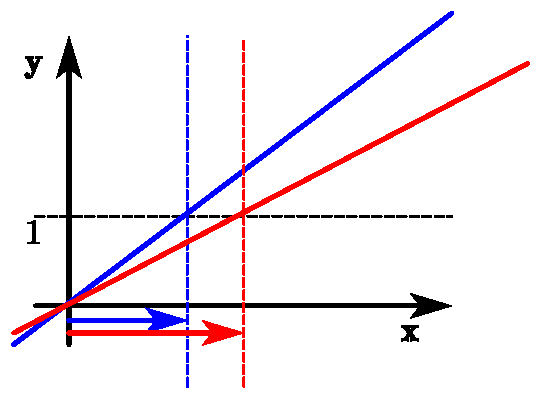
\includegraphics[width=8cm]{./figures/CoCon_1.pdf}
\caption{$V_1$和其偶空间$V_2$的基底关联示意图.蓝色和红色的箭头分别表示$x$轴上的两个向量,作为$V_1$的两个不同的基;蓝色和红色的实线代表两个不同的正比例函数,作为$V_2$的两个不同的基.两个空间的基的关联规则是,$V_1$的基被$V_2$的基映射到$1$上.可见,红色箭头比蓝色箭头长,但是红色函数的斜率比蓝色函数小,函数斜率和箭头长度呈现“逆变”关系.} \label{CoCon_fig1}
\end{figure}

现在,按照本节\autoref{CoCon_ex1} 中对偶空间的例子所定义的基底的关联,如果$V_1$的基向量是$\bvec{e}_1$,那么其所关联的$V_2$的基向量就是$f_1$,其中$f_1{\bvec{e}_1}=1$.$\bvec{e}_1$的选择是任意的,但$f_1$的选择要按照这个关联来确定;当然也可以反过来,任意选择$f_1$后再按照关联确定$\bvec{e}_1$.如果现在换用新的$V_1$的基向量$\bvec{e}_1'$,其中$\bvec{e}_1'=c\bvec{e}_1$,那么其所对应的$f_1'=f_1/c$.也就是说,$V_1$的基向量长度变为原先的$c$倍后,$V_2$的基向量长度(函数的斜率)变为原来的$1/c$倍.这样一来,$V_1$中每个元素的坐标都变为原来的$1/c$倍,而$V_2$中每个函数的斜率都变为原来的$c$倍.因此对偶空间彼此呈现\textbf{逆变}的关系.

将以上讨论的一维线性空间及其对偶的情况,推广到$n$维线性空间及其对偶,将数字$c$和$1/c$用矩阵$\bvec{Q}$和$\bvec{Q}^{-1}$代替,那么就得到一般情况下的线性空间及其对偶的逆变关系.

\subsection{张量的协变和逆变}
\pentry{张量的坐标变换\upref{TrTnsr}}

为了不失一般性,张量的定义极为抽象,只要求它是多个同构的线性空间上的多重线性映射.这些线性空间尽管彼此同构,其基底的选择却是彼此独立的.



%待续.睡觉去了.











